\section{IPS-N Drake}

\begin{center}
    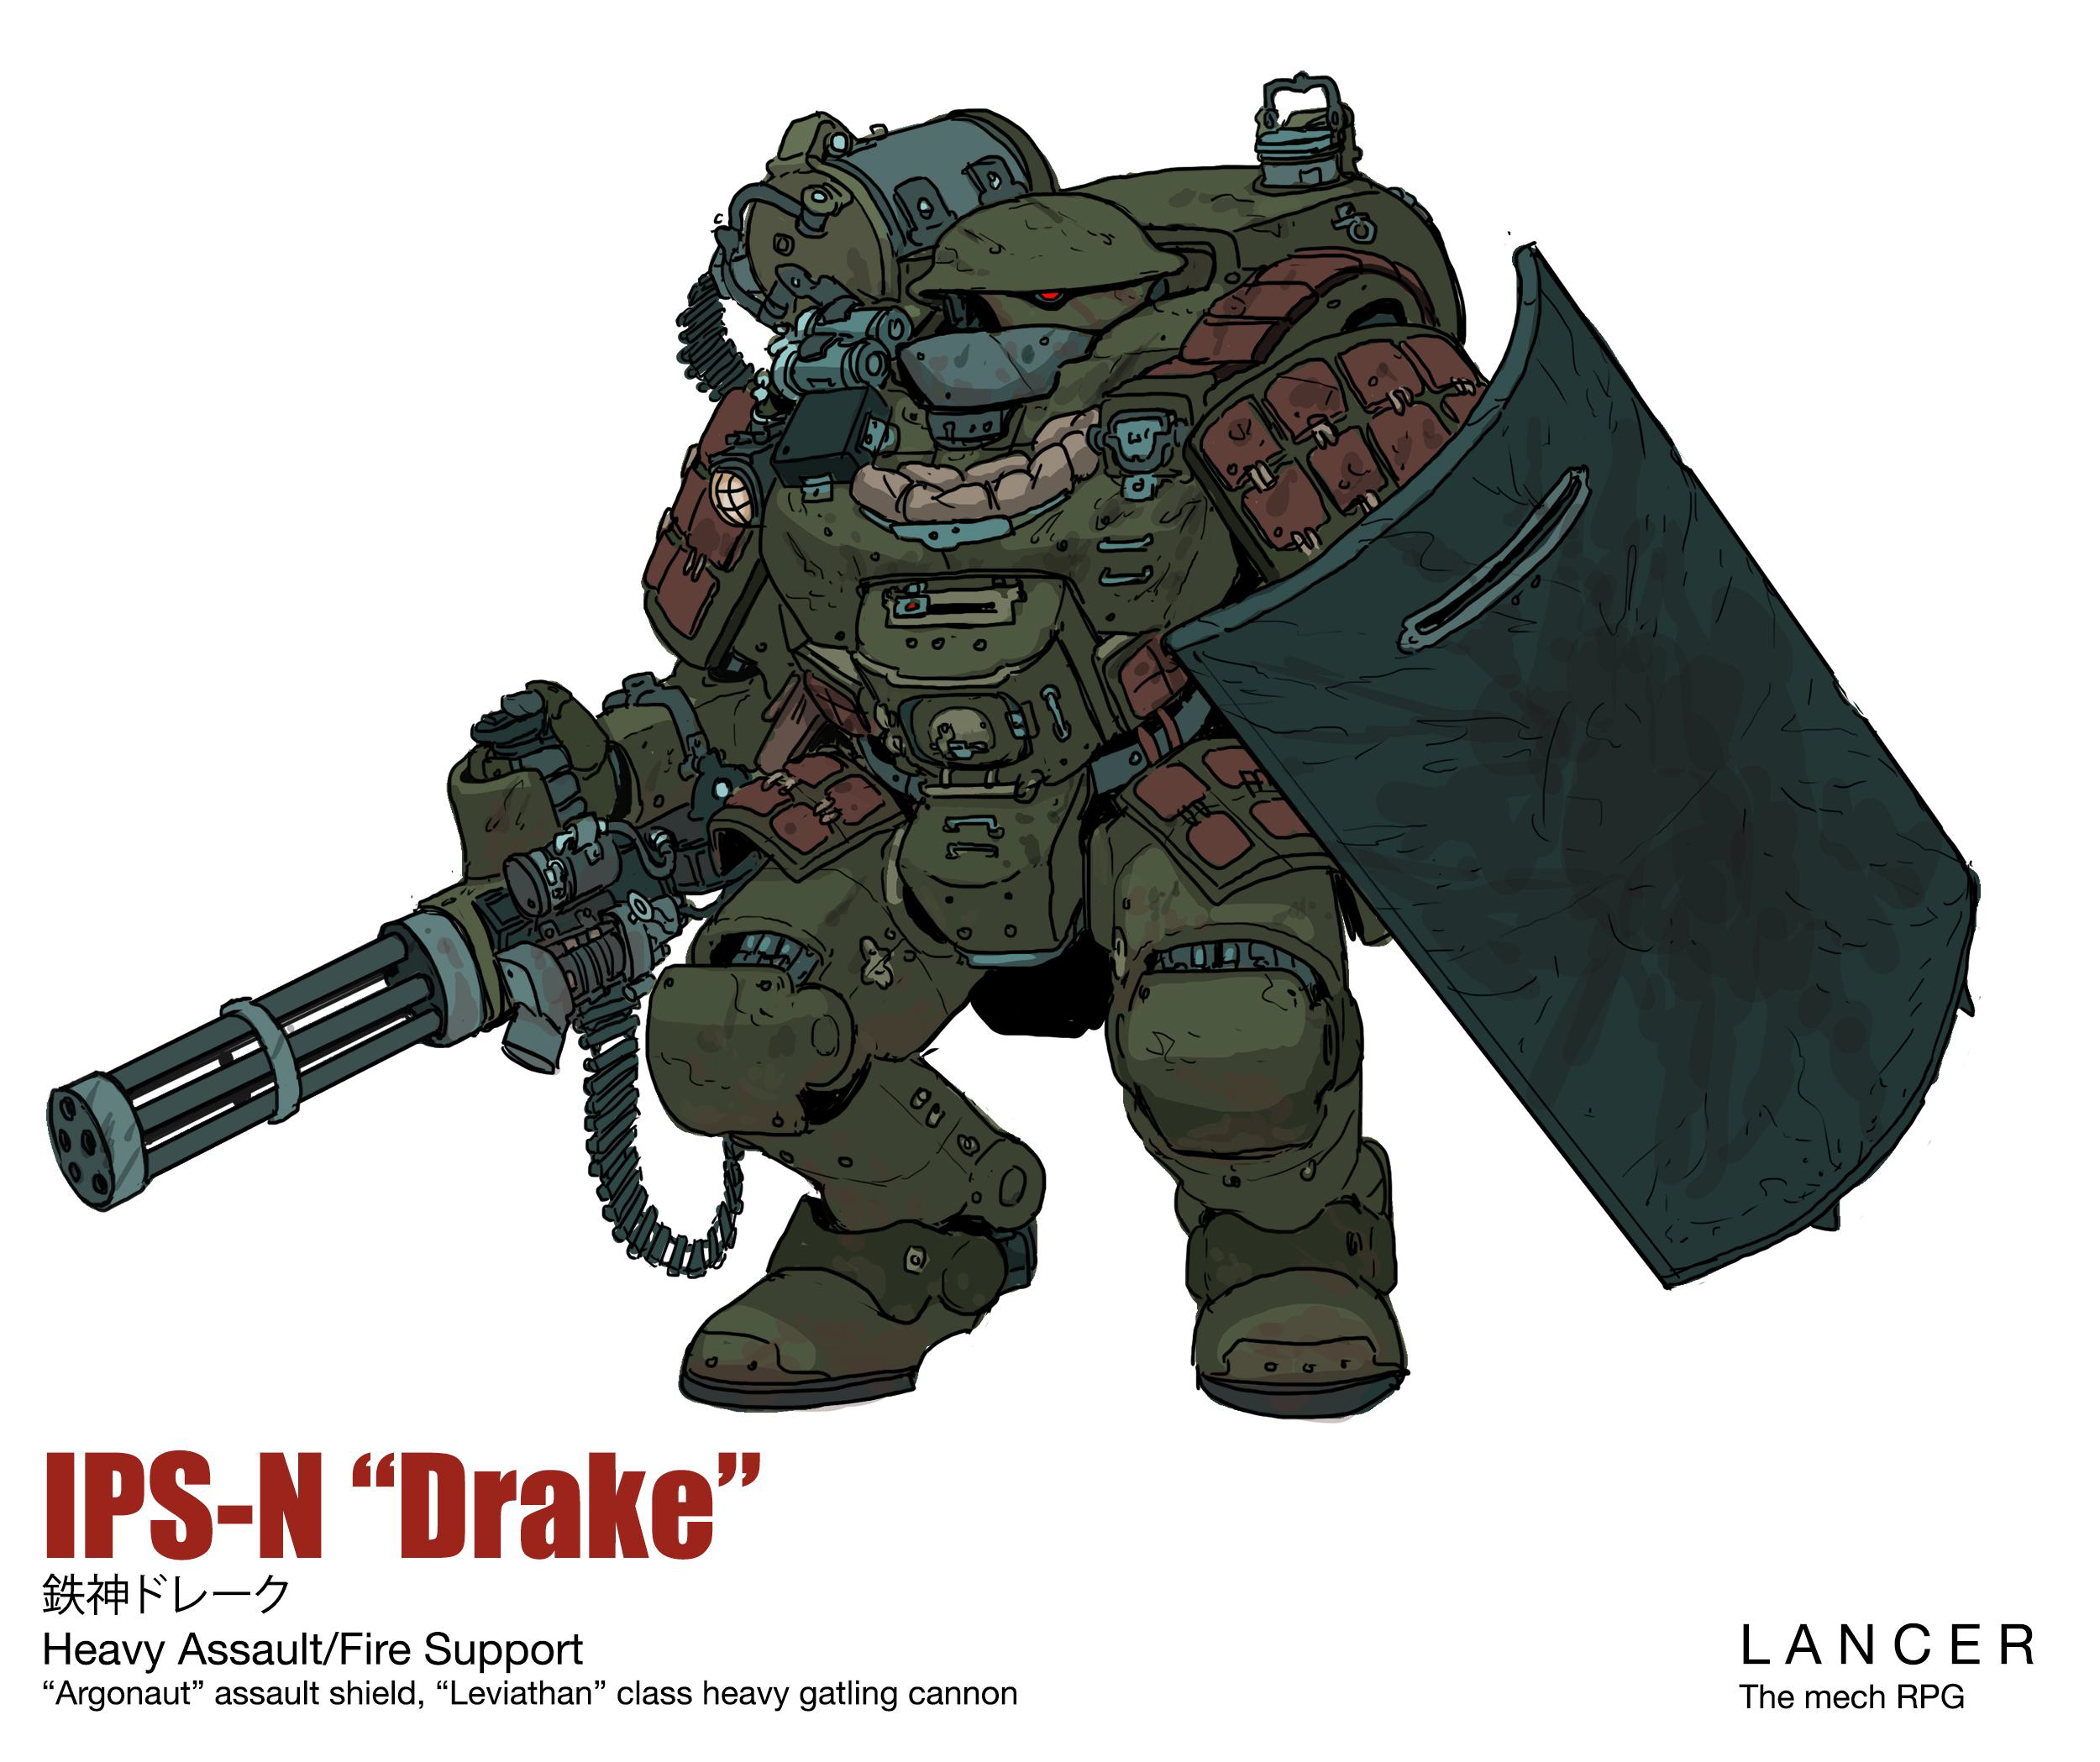
\includegraphics{Drake}
\end{center}


                                                    IPS-N DRAKE

The IPS-N DRAKE is the backbone of any proactive trade security/anti-piracy force and represents the
manufacturers first foray into military-grade mechs. It is a massive frame, simian in appearance, built
around a single-cast bulkhead sloped and reinforced to handle sustained incoming and outgoing fire.

A dense heavily armored chassis, the standard IPS-N DRAKE fleet license includes a high-velocity, high-
fragment assault cannon for suppressing and overwhelming their targets, and a heavy kinetic/ablative

barrier shield for defense. More advanced models feature scaled-up weaponry and armor, including the
notorious multi-barrel Leviathan cannon.




                                                     License:

I. Assault Cannon, Concussion Missiles

II. DRAKE FRAME, Aegis Shield Generator, IPS-N Argonaut Shield

III. Portable Bunker, Leviathan Heavy Assault Cannon


                                                     DRAKE

  HP: 8           Evasion: 6                             Speed: 3            Heat Cap: 5        Sensors: 10

  Armor: 3        E-Defense: 6                           Size: 2             Repair Cap: 4      Tech Attack:
                                                                                                +0

                                                     TRAITS:

  Heavy Frame: The Drake cannot be knocked back or prone by actors smaller than itself

  Blast Plating: The Drake has resistance to damage from blast, line, and cone attacks

  Guardian: Allied actors adjacent to the Drake gain Light Cover

  Slow: The Drake has +1 Difficulty on agility checks

                                               SYSTEM POINTS: 5

                                                    MOUNTS:

  Main Mount                         Main Mount                              Heavy Mount

                                          CORE SYSTEM: FORTRESS

  Active (requires 1 Core Power):
  Protocol

  When you activate this protocol, you plant your shield and deploy stabilizers, becoming more like a
  fortified emplacement than a mech. While this system is active, your mech is immobilized. Two line 2
  sections of heavy cover unfold, drawn from your mech in any direction. Your mech grants and benefits
  from heavy cover for allied mechs while this system is active and also grants any allies that benefit from
  this cover its immunity to knockback, prone, and resistance to blast, line, and cone attacks. This
  system can be deactivated at the start of your turn but cannot be reactivated without more core power.

Assault Cannon

The IPS-N assault cannon is a deep-cooled autocannon, able to be fielded as a fixed weapon or
manipulator-compatible platform. This autocannon can be fed by box-magazine or belt, is simple in its

functionality, and is a mainstay among IPS-N chassis fleet orders.

Main Cannon

1 heat (self), Overcharged

Range 8

1d6+2 Kinetic Damage





Concussion Missiles
Main Launcher

Range 5

Knockback 2

1d3 explosive damage

Targets struck by these missiles must pass a hull check or become impaired until the end of their
next turn.


Aegis Shield Generator

The Aegis is a portable electromagnetic shield generator, a way to establish a momentary safezone to

withstand an incoming bombardment or environmental hazard.

2 SP, Unique, Limited (1)
Shield, Deployable, Quick Action
Once planted in a free adjacent space, this size 1 generator creates a burst 2 zone around it until
the end of the current scene. All allied targets at least partly covered by the zone gain +1 armor
(up to 4). The generator has 10 HP but benefits from its own armor bonus, and deactivates once
used up.


IPS-N Argonaut Shield

2 SP, Quick Action
As a quick action, this heavy over-arm shield can be used to protect an adjacent actor from
incoming fire, giving them resistance to all damage as long as they stay adjacent to you.
However, your mech takes the half that was resisted. The effect breaks if they break adjacency,
and you must repeat this action to regain the effect.


Portable Bunker


A simple deployable, the “Portable Bunker” is actually a series of unfolding single-use printer sheets: flat-

pack pouches of inert non-newtonian fluid that, when deployed, are triggered into a rigid structure capable
of withstanding incredible force.

2 SP, Limited (1)
Deployable, Quick Action

To activate this system, choose a clear 4x4 space adjacent to you and take a quick action. At the
start of your next turn, this system unfolds into a fortified emplacement that grants heavy cover
to anyone within the area from all directions, as long as they are fully covered by the area. Actors
inside also have resistance to damage from blast, line, and cone attacks that originate from
outside the bunker.


The bunker is open topped and can be entered and exited at will. If attacked the bunker has
evasion 5 and 40 HP. It cannot be moved or deactivated once deployed.





Leviathan Heavy Assault Cannon

The Leviathan AC is a massive rotary autocannon, an enclosed multi-barrel automatic weapon fed by an

external reservoir, usually dorsally mounted on the chassis carrying it. At its current chambering, the
Leviathan should only be fired on automatic when absolutely necessary; IPS-N is currently working on a
solution to meet the cannon’s needs remotely. IPS-N recommends outfitting willing squadmates with extra

reservoirs, should their chassis have room to support it.

Superheavy Cannon

2 heat (self)

Range 8

1d6 kinetic damage


Unlike other superheavies, this weapon can be fired as part of a skirmish action with its listed
profile.

As a quick action, you can spin up this weapon’s barrels. While this weapon’s barrels are
spinning, your mech is Slowed, but this weapon’s damage increases to 4d6+4 kinetic, it must be
fired with a barrage action like a regular superheavy, and it gains Reliable 4. You can stop the
spin-up as a free action at the start of your turn, but lose the increased damage until you spin the
weapon up again.
